






Dans cette partie, nous allons raffiner les cas d’utilisation prioritaires et les
décrire en détail afin de mieux visualiser notre application.



\subsubsection{ Diagramme de cas d'utilisation "G\'{e}rer une tache"}
D\'{e}tailler le cas d'utilisation \guillemotleft{}G\'{e}rer un projet \guillemotright{} revient \`{a} d\'{e}tailler son propre
cas d'utilisation ainsi que ses 4 sous cas d'utilisation \`{a} savoir :

\begin{itemize}
\item{ G\'{e}rer un projet.}
\item{ G\'{e}rer  un membre.}
\item{ G\'{e}rer un client.}
\item{ G\'{e}rer  une t\^{a}che.}
\end{itemize}

\subsubsection{ Diagramme de cas d'utilisation "G\'{e}rer un projet"}

\begin{figure}[H]
\center
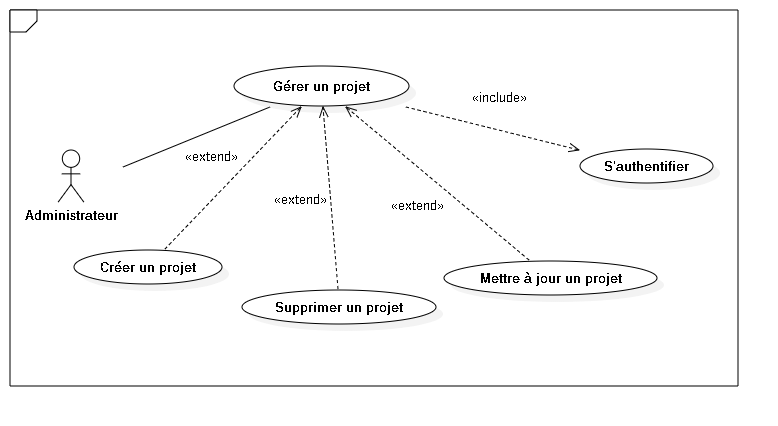
\includegraphics[width=13cm,height=8cm]{./figures/ucP.png}
\caption{G\'{e}rer un projet.}

\end{figure}



\subsubsection{ Diagramme de cas d'utilisation "G\'{e}rer un membre"}
\begin{figure}[H]
\center
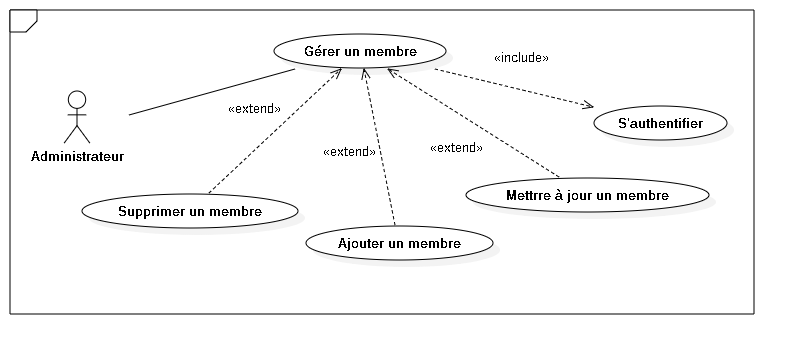
\includegraphics[width=13cm,height=8cm]{./figures/ucM.png}
\caption{G\'{e}rer un membre.}

\end{figure}


\subsubsection{ Diagramme de cas d'utilisation "G\'{e}rer un client"}
\begin{figure}[H]
\center
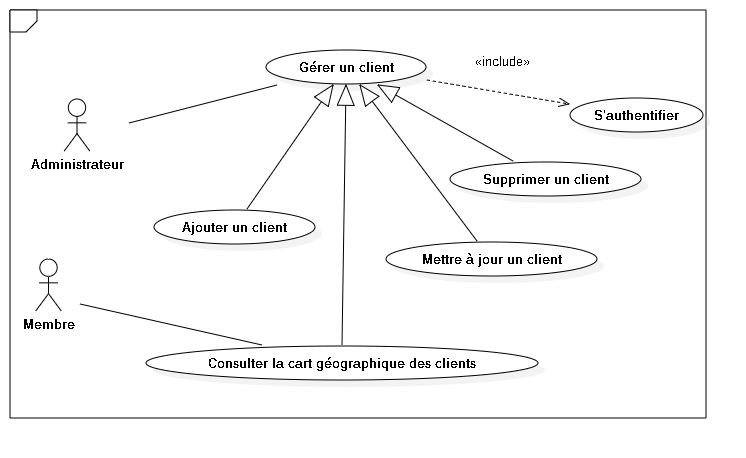
\includegraphics[width=13cm,height=8cm]{./figures/ucC.png}
\caption{G\'{e}rer un client.}
\end{figure}

\subsubsection{ Diagramme de cas d'utilisation "G\'{e}rer une t\^{a}che"}
\begin{figure}[H]
\center
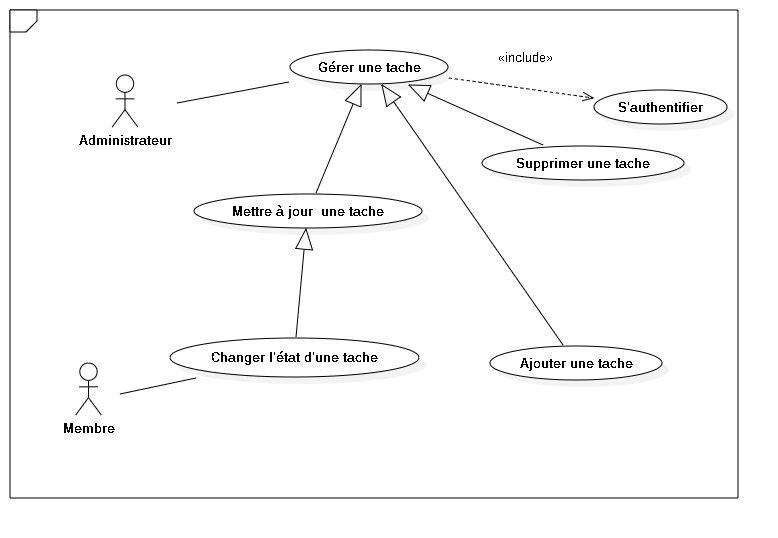
\includegraphics[width=13cm,height=8cm]{./figures/ucT.png}
\caption{G\'{e}rer une t\^{a}che.}

\end{figure}




